\section{The platforms that build system of e-commerce - Overview}
\label{sec:platform_overview}
The platforms that help build a system of e-commerce are exactly systems or portals that facilitate the life of a traded that want to start your own online business.
\newline
The process of setting up an online store with such systems is very fast and efficient, because essential information is easy to fit. The next moment is the choice of the graphical presentation of the store where the trader can choose from many themes and templates available.
These systems handle transparently different services that help create the store such as: the domain, payment management, organizing inventory, shipping and tracking of shipments, invoice management, etc.
\newline
The advantages and disadvantages of these platforms are mainly linked to the flexibility of the system itself. In fact, a platform for e-commerce-rich services, has more chance of being used by a growing number of major traded.
Obviously, a generic platform so can not meet the needs of every type of merchant because the platform has the purpose of facilitating the realization of a system of e-commerce in a more simple possibilie. Therefore it is difficult to meet the needs of each merchant from any kind of detail. Ease of use is another key point that leads to the platform to be chosen by dealers.
\newline
Following is shown the shopping cart technologies used by online stores globally. Last update Feb 24th 2016 \cite{commerce_platform_comparison}.
\begin{figure}[htb]
  \centering
  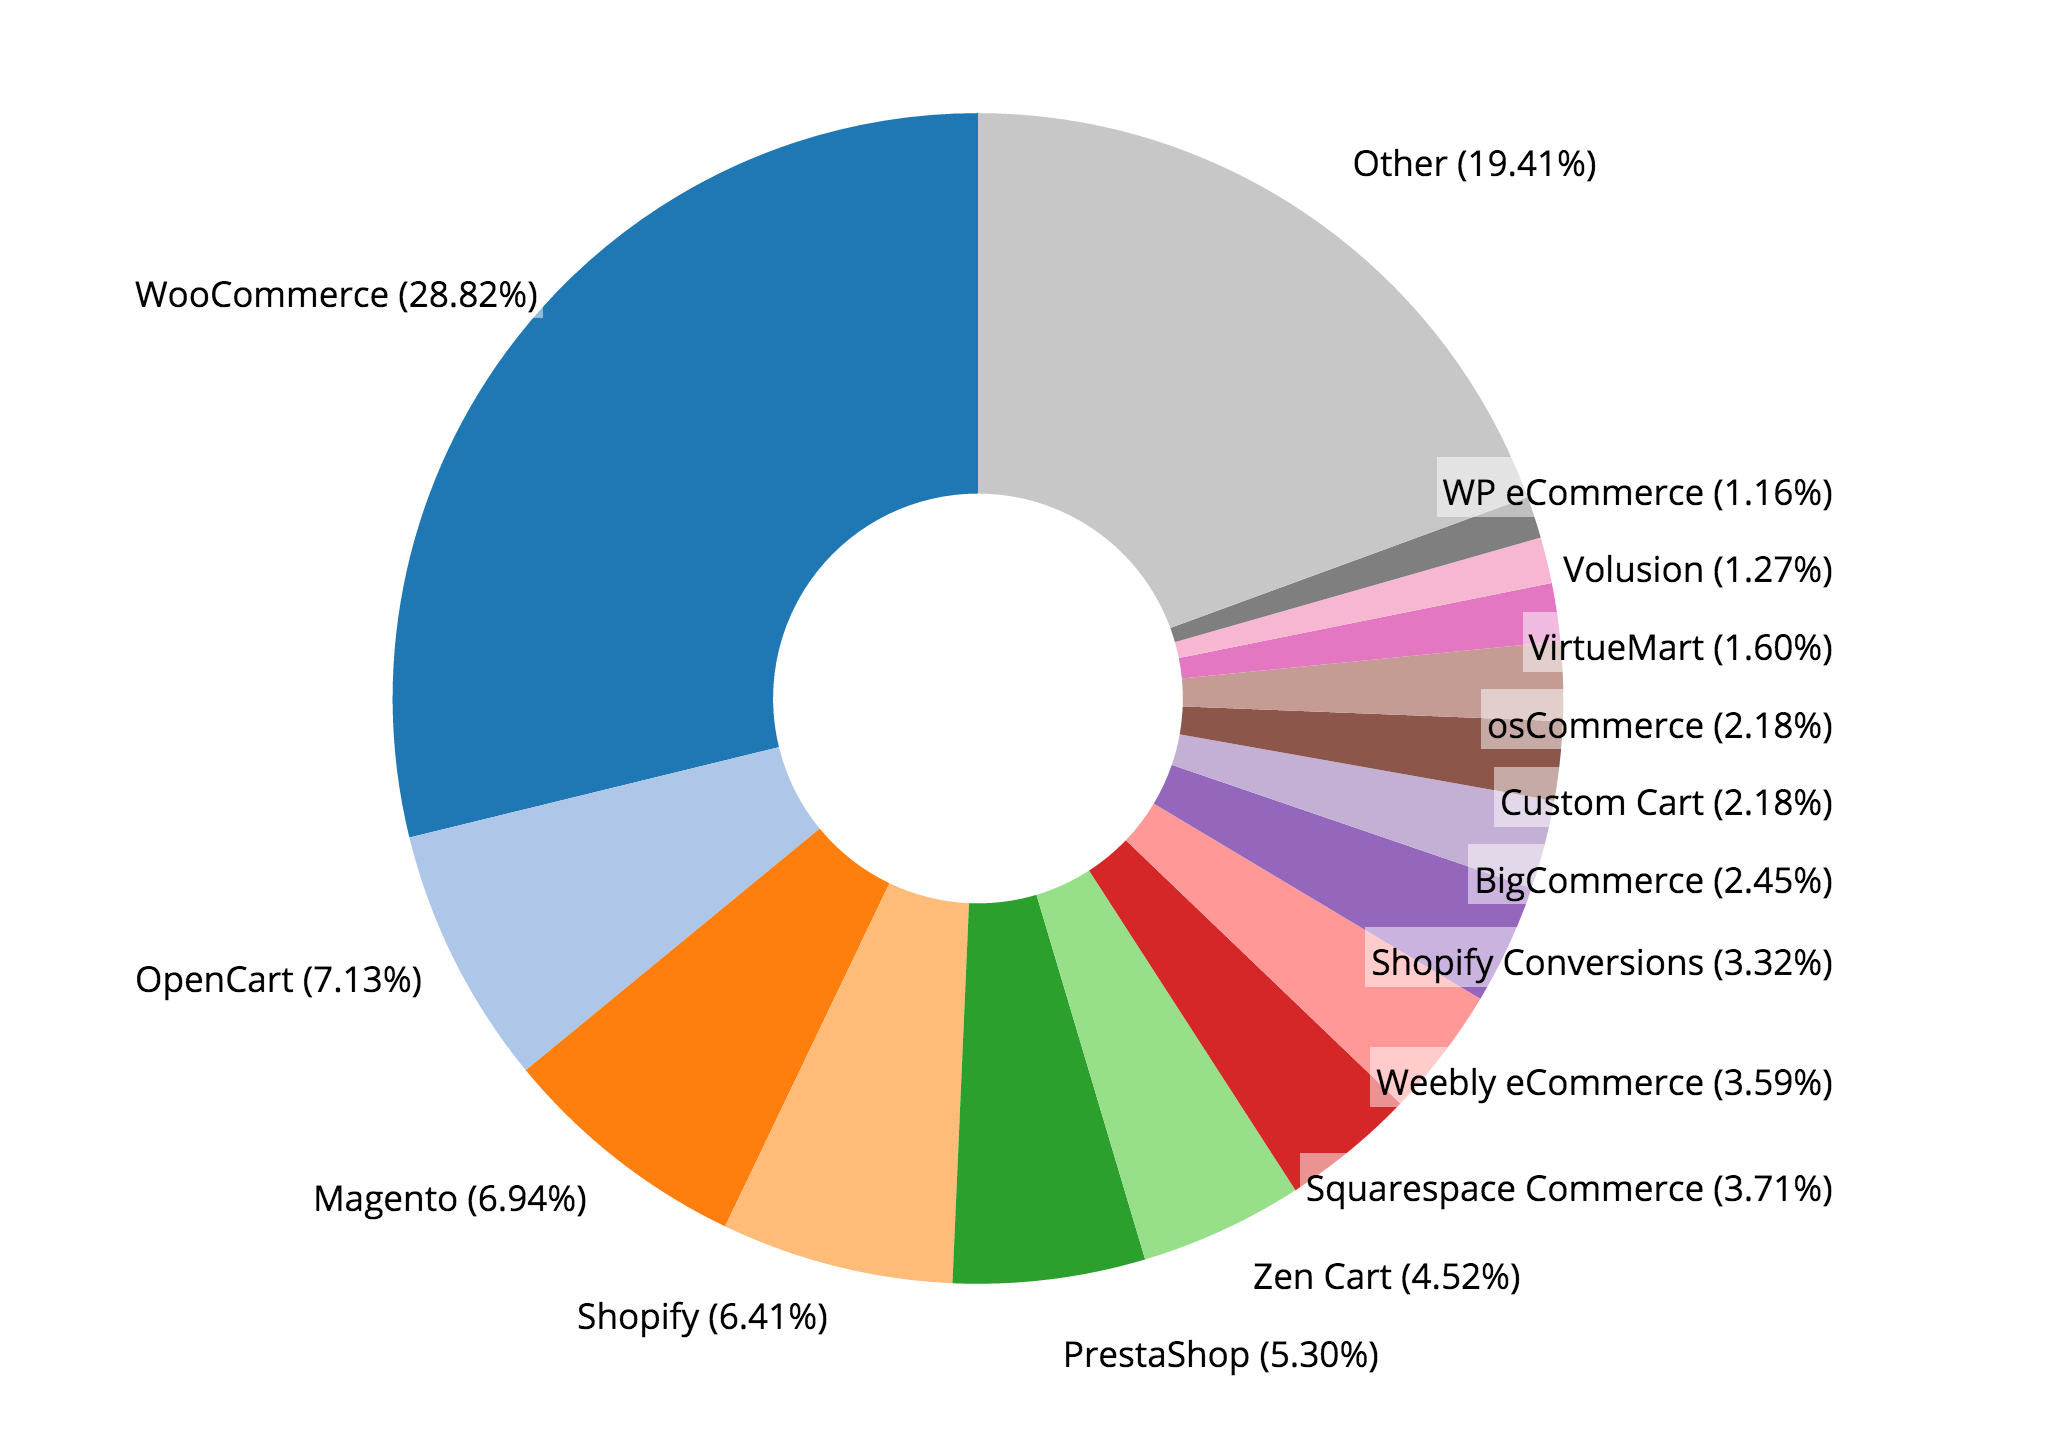
\includegraphics[width=0.8\linewidth]{images/chapter1/platform_comparison.png}\hfill
  \caption[Shopping cart technologies]{Shopping cart technologies}
  \label{fig:shopping_cart_technologies}
\end{figure}
\newpage
\subsection{Shopify}
Shopify is a Canadian commerce company headquartered in Ottawa, Ontario that develops computer software for online stores and retail point-of-sale systems \cite{shopify_overview}.
\begin{figure}[htb]
  \centering
  
\includegraphics[width=0.5\linewidth]{images/chapter1/shopify_logo.png}\hfill
  \caption[Shopify logo]{Shopify logo}
  \label{fig:ebay_logo}
\end{figure}
Shopify was founded in 2004, and was initially based on earlier software written by its founders for their online snowboard store. The company reports that it has 200,000 merchants using its platform, with total gross merchandise volume exceeding \$10 billion.
\newline
Shopify was founded in 2004 by Tobias Lütke, Daniel Weinand, and Scott Lake after attempting to open Snowdevil, an online store for snowboarding equipment. Unsatisfied with the existing e-commerce products on the market, Lütke, a programmer by trade, decided to build his own.
Lütke used the open source web application framework. Ruby on Rails to build Snowdevil's online store, and launched it after two months of development The Snowdevil founders launched the platform as Shopify in June 2006.
In September 2015, Amazon announced it would be closing its Amazon Webstore service for merchants, and had selected Shopify as the preferred migration provider. Shopify's shares jumped more than 20\% upon the news.
\begin{figure}[htb]
 \centering
 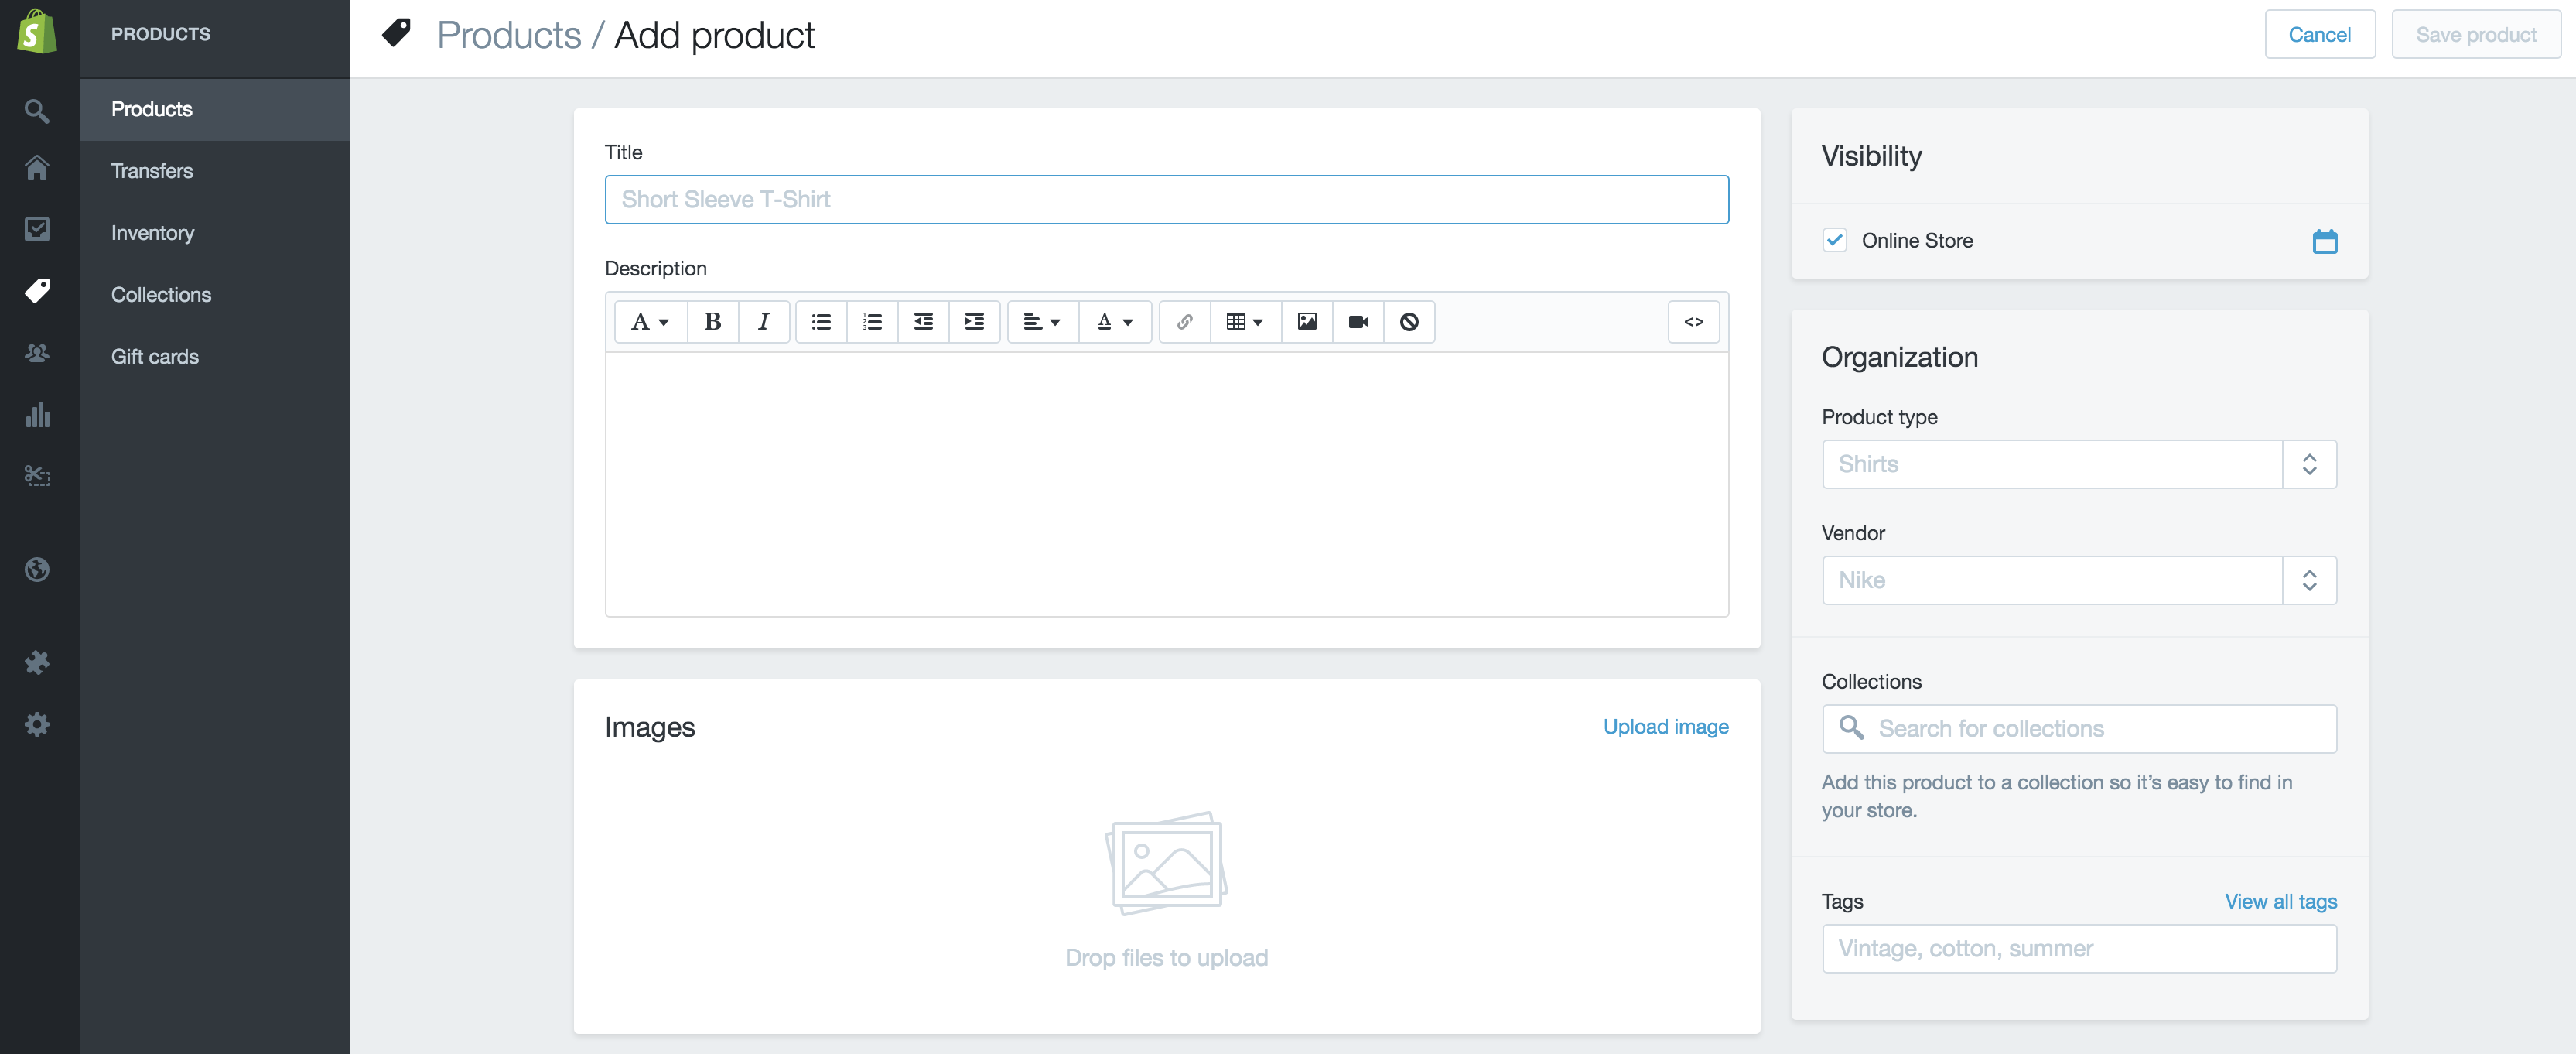
\includegraphics[width=1.0\linewidth]{images/chapter1/ex-shopify.png}\hfill
 \caption[Shopify Dashboard]{Shopify Dashboard}
 \label{fig:shopify_dashboard}
\end{figure}
\subsection{Bigcommerce}
Bigcommerce is a privately held technology company that develops e-commerce software for businesses. The company was founded in 2009 and has 370 employees with headquarters in Austin, Texas and additional offices in San Francisco, California and Sydney, Australia \cite{bigcommerce_overview}.
The company reports that \$5 billion in total sales have been processed by the Bigcommerce platform.
\begin{figure}[htb]
  \centering
  
\includegraphics[width=0.5\linewidth]{images/chapter1/bigcommerce_logo.jpg}\hfill
  \caption[Bigcommerce logo]{Bigcommerce logo}
  \label{fig:ebay_logo}
\end{figure}
Bigcommerce was founded in 2009 by Australians Eddie Machaalani and Mitchell Harper following a chance meeting in an online chatroom in 2003. In August 2009, the two relaunched a hosted version of Interspire Shopping Cart called “BigCommerce” and opened its first U.S. office.
\newline
Bigcommerce was 100\% bootstrapped until July 31, 2011, when it closed \$15 million in Series A funding from General Catalyst Partners. At the time, the company announced its client count had grown 680\% year over year. In January 2012, Bigcommerce launched a \$2 million integration fund for developers, which was used to fund 31 applications in the Bigcommerce App Marketplace. The company subsequently received \$20 million in Series B financing in September 2012, led by General Catalyst Partners and Floodgate Fund.
\begin{figure}[htb]
 \centering
 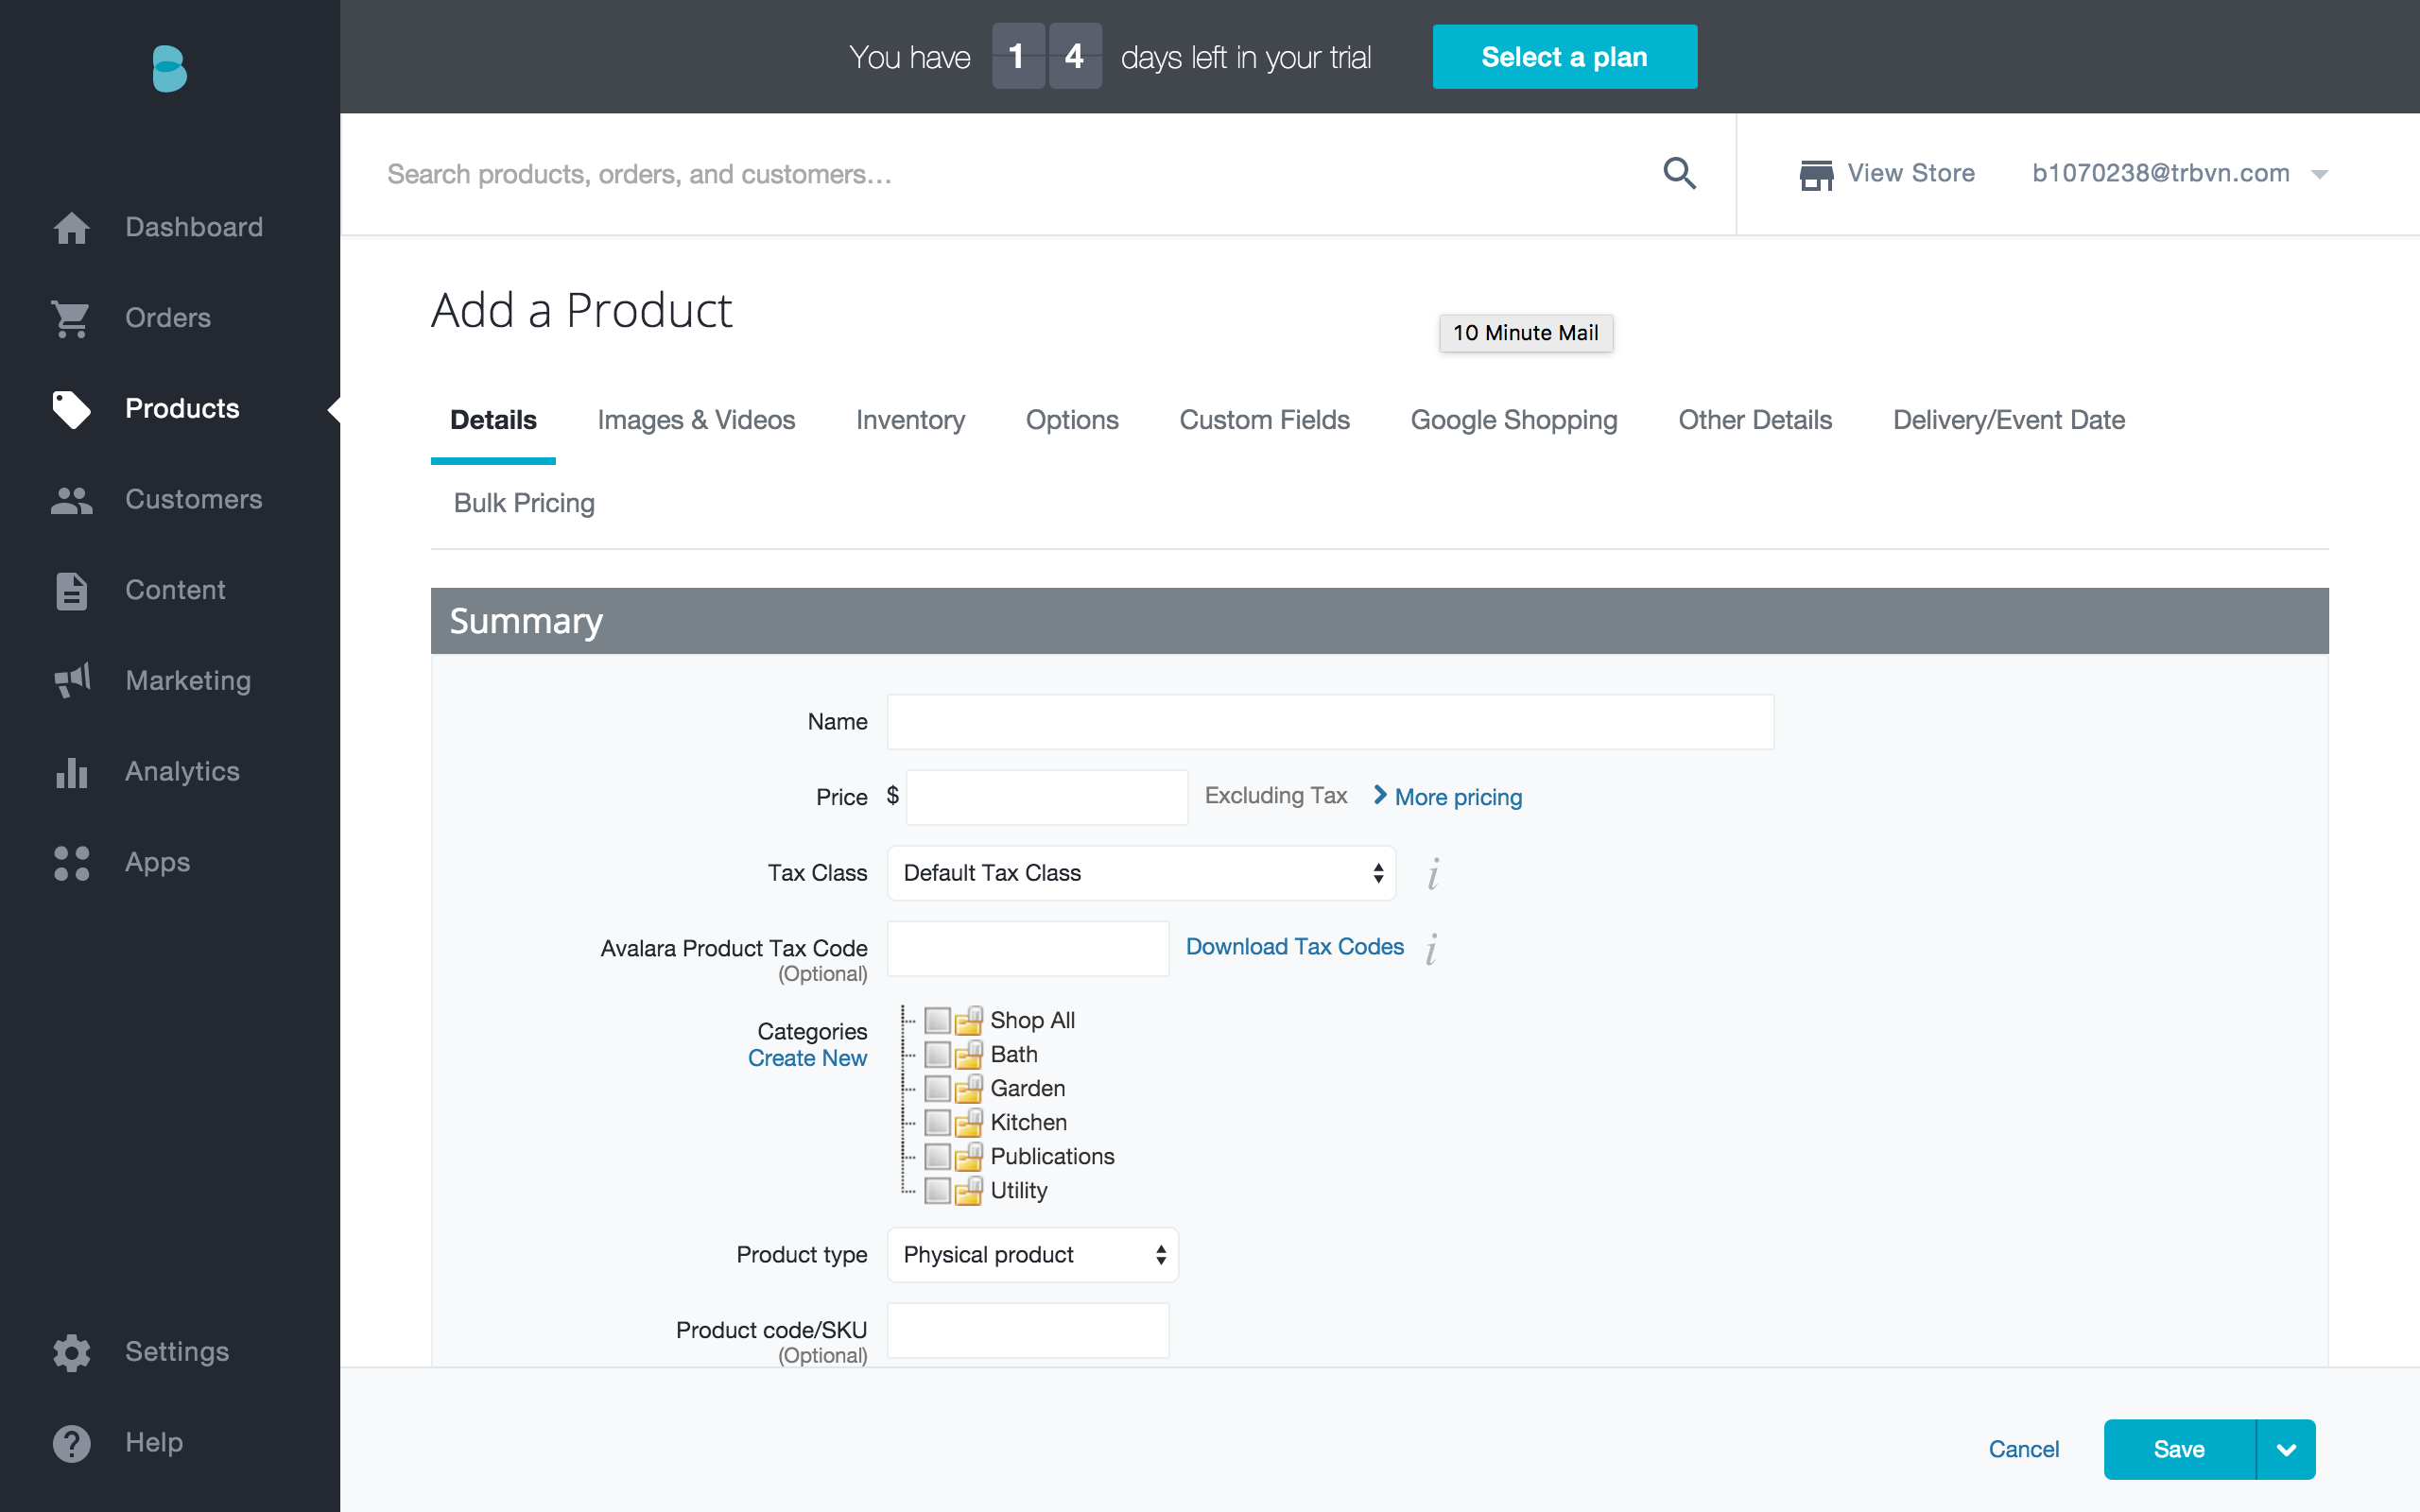
\includegraphics[width=1.0\linewidth]{images/chapter1/ex-bigcommerce.png}\hfill
 \caption[Bigcommerce Dashboard]{Bigcommerce Dashboard}
 \label{fig:shopify_dashboard}
\end{figure}

\subsection{Prestashop}
PrestaShop is a free, open source e-commerce solution and provides more than 250,000 online store owners with the most powerful, dynamic and international ecommerce software enriched with hundreds of innovative tools to build and manage a successful online store at no cost. PrestaShop is simple, efficient and intuitive with unmatched power that enables users to thrive in a competitive market regardless of size, industry or revenue \cite{prestashop_overview}.
\begin{figure}[htb]
  \centering
  
\includegraphics[width=0.5\linewidth]{images/chapter1/prestashop_logo.png}\hfill
  \caption[Prestashop logo]{Prestashop logo}
  \label{fig:ebay_logo}
\end{figure}
Used in over 200 countries and partnered with the most renowned names in the industry, PrestaShop continues to revolutionize online retail with technology that increases sales and maximizes visibility. Working hand in hand with its growing community of more than 850,000 dedicated members, PrestaShop’s entrepreneurial team is made up of ecommerce enthusiasts that are committed to the success and profitability of their online merchants.
PrestaShop started in 2005 as a student project within the EPITECH IT School in Paris, France. Originally named phpOpenStore, the software was first available in two languages: English and French. Three months after its launch the project was translated in thirteen languages.
\begin{figure}[htb]
 \centering
 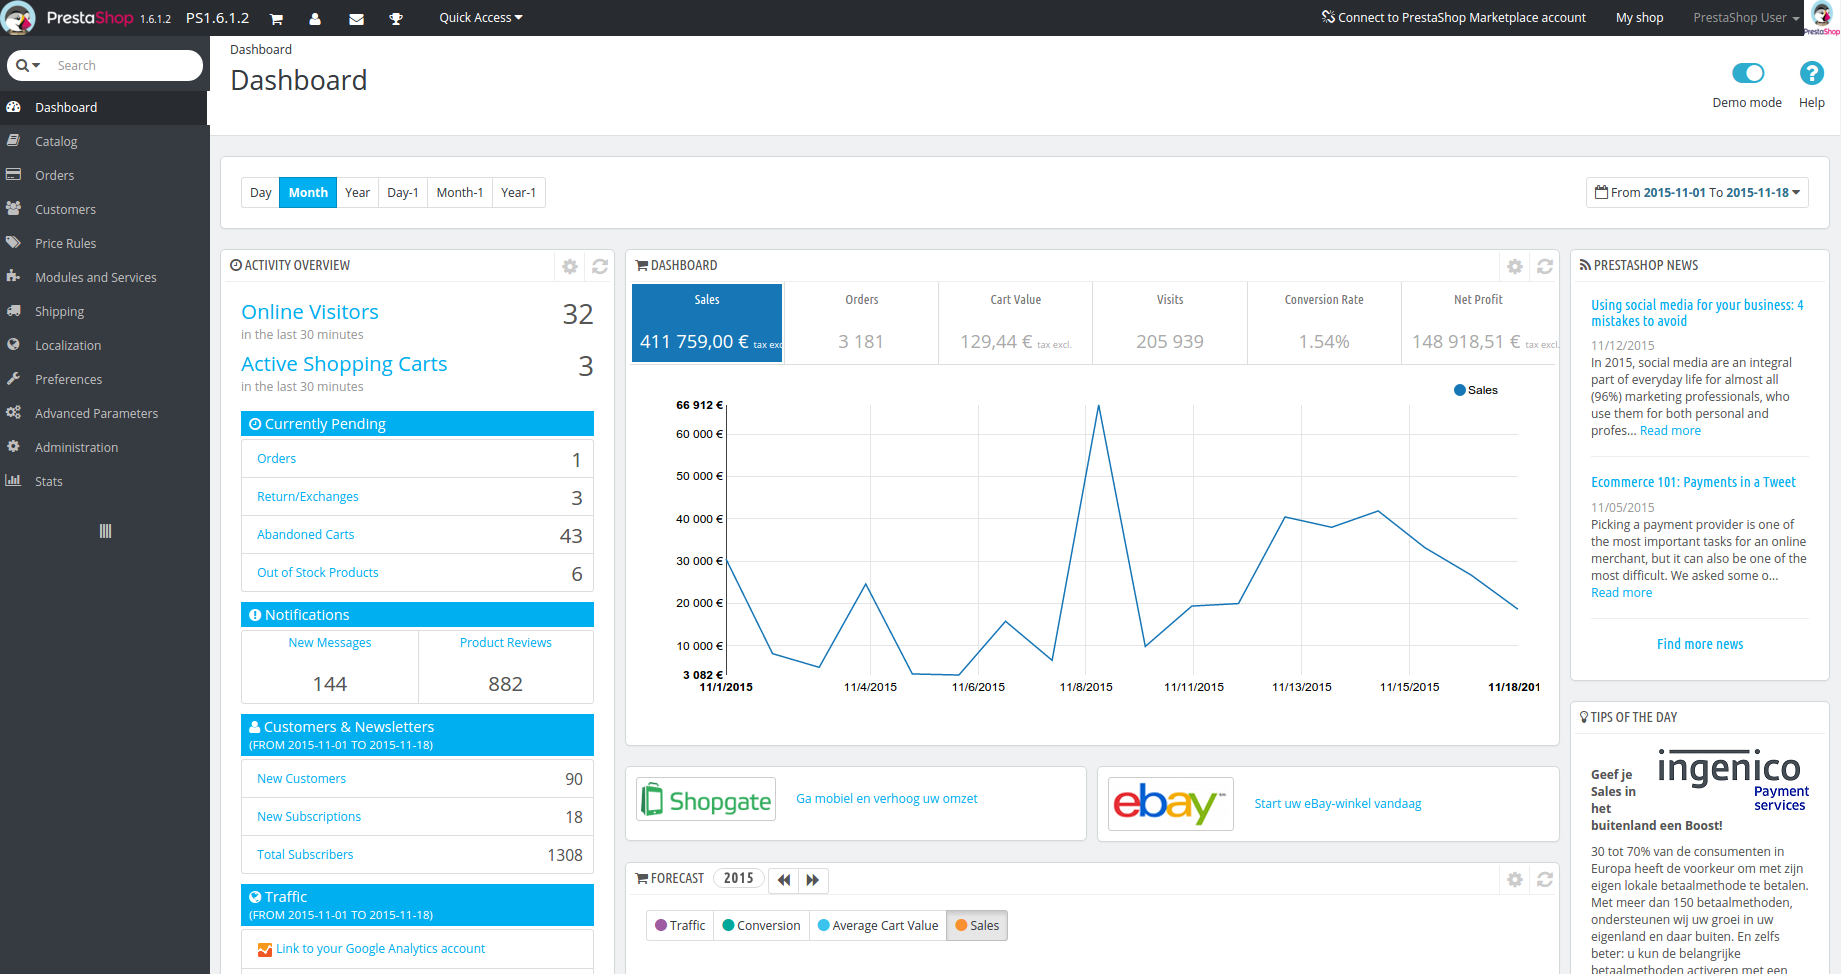
\includegraphics[width=1.0\linewidth]{images/chapter1/ex_prestashop.png}\hfill
 \caption[Prestashop Dashboard]{Prestashop Dashboard}
 \label{fig:prestashop_dashboard}
\end{figure}
The company, PrestaShop SA, was founded in 2007 by Igor Schlumberger and Bruno Lévêque. Between May 2010 and April 2012, PrestaShop grew from 17 employees to more than a hundred, with the establishment of secondary headquarters in Miami. In March 2014, PrestaShop SA secured \$9.3M in Series B Funding to continue its global expansion efforts. In January 2015, the company launched PrestaShop Cloud, a free self-hosted version of its software. According to technology tracking website BuiltWith.com, the market share of PrestaShop for open-source e-commerce websites is 9\%. According to W3Techs, PrestaShop is used by 0.5 of all websites \cite{prestashop_history}.